{{算法要求:}}

{① 必须采用顺序存储结构;}

{② 必须按关键字大小有序排列。}

{{基本思路:}首先,假设表中元素是按升序排列,将表中间位置记录的关键字与查找关键字比较,如果两者相等,则查找成功;否则利用中间位置记录将表分成前、后两个子表,如果中间位置记录的关键字大于查找关键字,则进一步查找前一子表,否则进一步查找后一子表。重复以上过程,直到找到满足条件的记录,使查找成功,或直到子表不存在为止,此时查找不成功。对应代码也并不难,如下:}

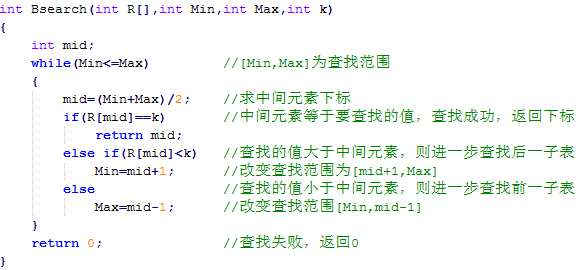
\includegraphics[width=3.70833in,height=1.72917in]{png-jpeg-pics/528BA045C8243E9DF3749442524992A9.png}
